\documentclass{standalone}
\usepackage{circuitikz}
\usepackage{tikz}
\usetikzlibrary{positioning}

\begin{document}


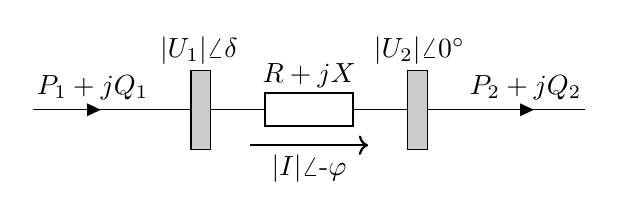
\begin{tikzpicture}
\draw (-1.5,0) to [short, i=$P_1+j Q_1$] (0,0) to [short] (1,0) to [european resistor, l=$R+j X$] (3,0) to [short] (4,0) to [short, i=$P_2+j Q_2$] (5.5,0);
\filldraw[fill=black!20!white, draw=black] (0.5,-0.5) rectangle (0.75,0.5);
\filldraw[fill=black!20!white, draw=black] (3.25,-0.5) rectangle (3.5,0.5);
\node[align=left] at (0.6,0.75) {$|U_1| \angle \delta$};
\node[align=left] at (3.4,0.75) {$|U_2| \angle 0^{\circ}$};
\draw[->, thick] (1.25,-0.45) to (2.75,-0.45);
\node[align=left] at (2,-0.75) {$|I| \angle \textrm{-}\varphi$};
\end{tikzpicture}

\end{document}